\problemname{Long-Exposure Photography}
Gwen has painted some rectangles with completely black surfaces on a large sheet of graph paper.
To ensure that everything looks neat and tidy, all of her rectangles' edges lie on the lines of the paper.
Now she intends to take a photo of the paper while spinning it very fast.
The exposure time of the camera is long enough to cover an entire rotation of the plane.
In the resulting photo, areas covered by rectangles throughout the entire rotation will appear black, whereas areas never covered by a rectangle will appear white.
The remaining ``blurry'' areas may vary in brightness, but Gwen simply considers all of those to be grey.

Now, before taking the photo, Gwen tells you the coordinates of the rectangles she has painted and asks you to determine how much of the photo's surface area will be black and how much of it will be grey.

\vspace{-.2cm}
\begin{figure}[!h]
	\centering
	\begin{subfigure}{}
		\raisebox{-0.5\height}{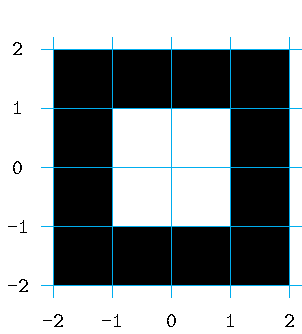
\includegraphics[scale=0.9]{samplein}}
	\end{subfigure}
	\hspace{1cm}
	\begin{subfigure}{}
		\raisebox{-0.5\height}{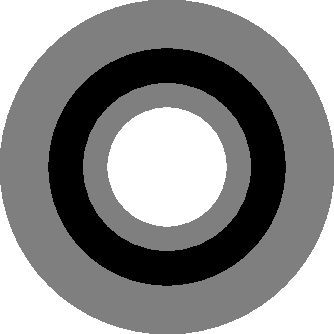
\includegraphics[scale=0.9]{sampleans}}
	\end{subfigure}
	\caption{The first sample input and the resulting photo.}
\end{figure}
\vspace{-1cm}

\section*{Input}
The input consists of:
\begin{itemize}
	\item One line with an integer $n$ ($1 \le n \le 1\,000$), giving the number of rectangles.
	\item $n$ lines, each with four numbers: two integers $x_{min}, y_{min}$ ($-10^9 \le x_{min}, y_{min} \le 10^9$) giving the coordinates of the rectangle's bottom left corner (that is, the corner with minimum x and y values) and two integers $w, h$ ($1 \le w, h \le 200$) giving the rectangle's width and height.
\end{itemize}
The plane is rotated around the origin $(0, 0)$, and you may safely assume that the entire sheet of paper is fully captured by the camera throughout the entire rotation.

\section*{Output}
Output two real numbers, the first being the area of the black and the second being the area of the grey portion of the photo's surface.
A number is considered correct if its absolute or relative error does not exceed $10^{-6}$.
